\documentclass[10pt,twocolumn]{article}
\usepackage[margin=0.68in,columnsep=0.24in]{geometry}
\usepackage[T1]{fontenc}
\usepackage[utf8]{inputenc}
\usepackage{lmodern}
\usepackage{microtype}
\usepackage{amsmath,amssymb,amsthm}
\usepackage{booktabs}
\usepackage{graphicx}
\usepackage{xcolor}
\usepackage{enumitem}
\usepackage{hyperref}

\hypersetup{
  colorlinks=true,
  linkcolor=blue!60!black,
  citecolor=blue!60!black,
  urlcolor=blue!60!black,
  pdftitle={Certified Verification of Alpha-Beta Pruning via Monadic Continuations},
  pdfauthor={Lluis Eriksson}
}

\newtheorem{proposition}{Proposition}

\title{\vspace{-1.1em}\textbf{Certified Verification of Alpha-Beta Pruning via Monadic Continuations}}
\author{Lluis Eriksson\thanks{Independent Researcher. Code, Lean~4 proofs, and certificates: MIT License; manuscript and figures: CC-BY-4.0. Prepared with AI coding, formalization, and drafting assistance from Google Antigravity; all proofs, exact discrete verifiers, and adversarial tests were independently compiled and verified locally. Repository: \url{https://github.com/lluiseriksson/alphabeta-monadic-continuations-certificates}}}
\date{November 25, 2026}

\begin{document}
\maketitle
\vspace{-1.4em}

\begin{abstract}
Mart{\'\i}n H{\"o}tzel Escard{\'o} and Paulo Oliva (\texttt{arXiv:2611.32320}, Nov.\ 2026) derived alpha-beta pruning purely functionally by embedding minimax into the continuation monad $K_R X = (X \to R) \to R$ paired with a Reader-carried $(\alpha,\beta)$ window, proving soundness (Thm.~1), strict-window exactness (Cor.~1(a)--(b)), and optimal-play extraction via first-element tie-breaking (Sec.~5, Cor.~2), including history-dependent Tic-Tac-Toe pruning from $9! = 362{,}880$ plays to $9{,}335$. We construct a standalone zero-dependency \textbf{Lean~4.35.0} formalization of 18 core theorems---including full mutually recursive inductive proofs of Lemma~2, Theorem~1, Corollaries~1(a)--(b) and~2, Reader/Continuation monad laws, tie-preserving \texttt{pickMax}/\texttt{pickMin}, and the exact Wikipedia 36-leaf tree (zero \texttt{sorry}, zero warnings, zero \texttt{Classical.choice})---paired with a zero-floating-point discrete verifier (\texttt{ALPHABETA-MONAD-CERT-1.0}). Across 16 canonical certificates ($0.092$--$103.002\,\mathrm{ms}$, total $124.66\,\mathrm{ms}$), all exact traces, aspiration-window regimes, Definition~2 optimal-play witnesses, and full Tic-Tac-Toe ($362{,}880 \to 9{,}335$, $38.873\times$) replay deterministically while rejecting 60/60 live adversarial forgery attacks.
\end{abstract}

\section{Introduction}\label{sec:intro}
Alpha-beta pruning~\cite{hart1961tree,knuth1975analysis} is a foundational game-tree optimization, yet unifying its imperative early cutoffs with compositional denotational semantics for sequential games~\cite{escardo2010selection,escardo2011sequential,escardo2023higher} has remained subtle, motivating recent selection-monad formulations~\cite{hartmann2025selection,hartmann2026alphabeta}. Escard{\'o} and Oliva~\cite{escardo2026alphabeta} resolve this cleanly without mutable state or exceptions via four linked mechanisms:
\begin{enumerate}[leftmargin=*,nosep]
  \item \textbf{Monadic Continuation Pruning (Sec.~2--3):} Lifting a game tree into the continuation monad $K_R X = (X \to R) \to R$ and threading $(\alpha,\beta)$ bounds via the Reader monad replaces exhaustive \texttt{max}/\texttt{min} over children with short-circuiting \texttt{takeUntil} folds that abort evaluation the moment a maximizer meets $\beta$ or a minimizer meets $\alpha$.
  \item \textbf{Theorem~1 \& Lemma~2 Soundness (Sec.~4):} For every finite tree $T$ and $\alpha < \beta$, the pruned value $v = \mathrm{ab}(T, \alpha, \beta)$ satisfies fail-low ($\mathrm{mm}(T) \le \alpha \Rightarrow v \le \alpha$), fail-high ($\mathrm{mm}(T) \ge \beta \Rightarrow v \ge \beta$), and exactness ($\alpha < \mathrm{mm}(T) < \beta \Rightarrow v = \mathrm{mm}(T)$), yielding Corollaries~1(a) (wide bounds) and~1(b) (in-window exactness).
  \item \textbf{Optimal Play Extraction \& Tie-Breaking (Sec.~5, Def.~2, Cor.~2):} Extending values to pairs $(v, \pi) \in \mathbb{Z} \times \mathrm{Play}$ requires strict tie-preserving comparisons (\texttt{pickMax} keeps the earlier move on equality $x \ge y$, and \texttt{pickMin} on $x \le y$) so pruned subgames returning a tied cutoff bound cannot displace a genuinely optimal earlier play.
  \item \textbf{History-Dependent Games \& Tic-Tac-Toe (Sec.~6):} Supporting variable-branching history-dependent move sets yields exact root-to-leaf Tic-Tac-Toe pruning from $9! = 362{,}880$ full plays to $9{,}335$ evaluated plays ($38.873\times$) with optimal draw play $[0,4,1,2,6,3,5,7,8]$.
\end{enumerate}

\paragraph{Contributions and Scope.}
We machine-check the complete discrete inductive theory of~\cite{escardo2026alphabeta} over arbitrary finite history-dependent \texttt{GameTree}s without floating-point arithmetic or classical axioms:
(i)~18 zero-\texttt{sorry}, zero-\texttt{Classical.choice} \textbf{Lean~4.35.0}~\cite{demoura2021lean4} theorems in \texttt{AlphaBetaMonadic.lean};
(ii)~the exact discrete verifier \texttt{ALPHABETA-MONAD-CERT-1.0};
(iii)~16 canonical certificates across all four verification modes; and
(iv)~a 60-attack live red-team suite with 39-artifact SHA-256 manifest enforcement.

\section{Constructive Lean~4.35.0 Kernel}\label{sec:lean}
The standalone module \texttt{AlphaBetaMonadic.lean} (in \texttt{lean/}) defines arbitrary finite \texttt{GameTree}s via \texttt{leaf (out : Outcome)}, \texttt{maxNode}, and \texttt{minNode} (with play sequences carried in leaf \texttt{Outcome}s), exhaustive minimax \texttt{out}/\texttt{outList}, first-order \texttt{takeUntil}-pruned \texttt{outAB}/\texttt{outABListMax}/\texttt{outABListMin}, leaf-membership \texttt{isLeafOutcome}, and standalone \texttt{Reader}/\texttt{Cont} monads. Using pure mutual structural recursion, it compiles under Lean~4.35.0 in $1.3\,\mathrm{s}$ with zero dependencies, zero warnings, and zero \texttt{sorry}. Auditing all 18 theorems via \texttt{\#print axioms} (\texttt{AuditAxioms.lean}) confirms 8 zero-axiom theorems (\texttt{none}), 10 using only \texttt{[propext, Quot.sound]}, and \textbf{0} using \texttt{Classical.choice} or \texttt{Lean.ofReduceBool} (Table~\ref{tab:lean}).

\begin{table}[t]
\centering
\caption{All 18 machine-checked Lean~4.35.0 theorems in \texttt{AlphaBetaMonadic.lean} (zero \texttt{sorry}, zero \texttt{Classical.choice}).}
\label{tab:lean}
\scriptsize
\setlength{\tabcolsep}{1.5pt}
\begin{tabular}{@{}rlll@{}}
\toprule
\# & Lean Theorem Identifier & Paper Ref. & Axioms \\
\midrule
1 & \texttt{pickMax\_val\_eq\_max} & Sec.~5 & \texttt{p, Q} \\
2 & \texttt{pickMin\_val\_eq\_min} & Sec.~5 & \texttt{p, Q} \\
3 & \texttt{pickMax\_first\_tie\_preserves} & Sec.~5 & \texttt{none} \\
4 & \texttt{pickMin\_first\_tie\_preserves} & Sec.~5 & \texttt{none} \\
5 & \texttt{takeUntil\_nonempty\_of\_nonempty} & Sec.~3.1 & \texttt{none} \\
6 & \texttt{takeUntil\_all\_false\_eq\_self} & Sec.~3.1 & \texttt{none} \\
7 & \texttt{takeUntil\_head\_ge\_stops} & Sec.~3.1 & \texttt{none} \\
8 & \texttt{reader\_monad\_laws} & Sec.~3.1 & \texttt{none} \\
9 & \texttt{continuation\_monad\_laws} & Sec.~2 & \texttt{none} \\
10 & \texttt{lemma2\_max\_fail\_low} & Lem.~2 & \texttt{p, Q} \\
11 & \texttt{lemma2\_max\_fail\_high} & Lem.~2 & \texttt{p, Q} \\
12 & \texttt{lemma2\_min\_fail\_high} & Lem.~2 & \texttt{p, Q} \\
13 & \texttt{lemma2\_min\_fail\_low} & Lem.~2 & \texttt{p, Q} \\
14 & \texttt{theorem1\_alphabeta\_soundness} & Thm.~1 & \texttt{p, Q} \\
15 & \texttt{corollary1a\_strict\_global\_bounds} & Cor.~1(a) & \texttt{p, Q} \\
16 & \texttt{corollary1b\_in\_window\_exactness} & Cor.~1(b) & \texttt{p, Q} \\
17 & \texttt{corollary2\_optimal\_play\_soundness} & Cor.~2 & \texttt{p, Q} \\
18 & \texttt{wikipedia\_example\_tree\_exact\_pruning} & Sec.~2.2 & \texttt{none} \\
\bottomrule
\end{tabular}
\vspace{-0.4em}
\begin{flushleft}
\tiny Axiom key: \texttt{none} = zero axioms (8); \texttt{p, Q} = \texttt{[propext, Quot.sound]} (10).
\end{flushleft}
\vspace{-0.8em}
\end{table}

\begin{proposition}[Machine-Checked Monadic Alpha-Beta Invariants]\label{prop:lean}
The Lean~4.35.0 kernel establishes the following universal results over arbitrary finite \texttt{GameTree}s and integer payoffs:
\begin{enumerate}[leftmargin=*,nosep]
  \item \emph{Monad, Cutoff, \& Tie-Breaking Laws (Thms.~1--9):} \texttt{Reader} and \texttt{Cont} satisfy all three monad laws; \texttt{takeUntil} preserves non-emptiness and stops immediately on cutoff; \texttt{pickMax}/\texttt{pickMin} compute exact \texttt{max}/\texttt{min} values while deterministically preserving the first argument on ties.
  \item \emph{Soundness, Exactness, \& Optimal Plays (Thms.~10--18):} All four cases of Lemma~2 hold for arbitrary child lists, proving Theorem~1 for \texttt{outAB} by mutual induction on \texttt{GameTree}. Strict global bounds (Cor.~1(a)) and in-window outputs $\alpha < v < \beta$ (Cor.~1(b)) force $v = (\texttt{out } T).\texttt{val}$ and certify that the returned path is a genuine leaf witness via \texttt{isLeafOutcome} (Cor.~2). On the exact 36-leaf Wikipedia tree \texttt{wikiTree}, \texttt{out} and \texttt{outAB} both return $\langle 6, [1,0,0,0]\rangle$ (while the exact 18-leaf evaluation trace is certified in Mode~1).
\end{enumerate}
\end{proposition}

\section{Exact Discrete Certificate Verifier}\label{sec:cert}
The verifier \texttt{ALPHABETA-MONAD-CERT-1.0} (\texttt{src/alphabeta\_certifier.py}, \texttt{src/alphabeta\_exact.py}) uses pure Python \texttt{int} and exact finite game trees exclusively (source-audited for zero \texttt{float(}, \texttt{math.}, or \texttt{numpy}). Every payload enforces strict JSON typing (rejecting floats, bool-as-int, int-as-bool), nesting-depth cap $32$, full ASCII control-character filtering, 2048-bit integer caps, distinct non-empty move lists matching child counts, and exact container/key validation across four modes:
\begin{enumerate}[leftmargin=*,nosep]
  \item \textbf{Mode~1 (Sec.~2.2/3.3/5 Fixed-Tree Monadic Trace):} Replays both exhaustive minimax and monadic alpha-beta on the submitted tree, verifying exact minimax value/play, leaf counts, Theorem~1(i)--(iii) soundness, and the exact ordered leaf-evaluation trace.
  \item \textbf{Mode~2 (Thm.~1 \& Cor.~1(b) Window Stress Audit):} Evaluates multiple aspiration and boundary windows $(\alpha,\beta)$ on one tree, classifying every window into \texttt{exact\_window}, \texttt{fail\_low}, or \texttt{fail\_high}, checking Corollary~1(b), and auditing tie-preserving move selection.
  \item \textbf{Mode~3 (Def.~2 \& Cor.~2 Optimal Play Witness):} Independently walks the claimed play ply-by-ply against exact subgame minimax values at every internal node, certifying that every maximizer/minimizer step achieves its true minimax value.
  \item \textbf{Mode~4 (Sec.~6.2 History-Dependent Tic-Tac-Toe):} Replays exact monadic alpha-beta on $3\times 3$ Tic-Tac-Toe from any legal prefix (with optional exhaustive subgame check), certifying exact evaluated leaf counts, Corollary~1(b) in-window exactness, and optimal play completion.
\end{enumerate}

\section{Empirical Atlas and Red-Team Audit}\label{sec:results}
Running \texttt{run\_all\_experiments.py} generates 16 canonical certificates (4 per mode) and four exact datasets, audited end-to-end by \texttt{verify\_all.py} with SHA-256 verification across all 39 tracked artifacts.

\begin{figure}[t]
  \centering
  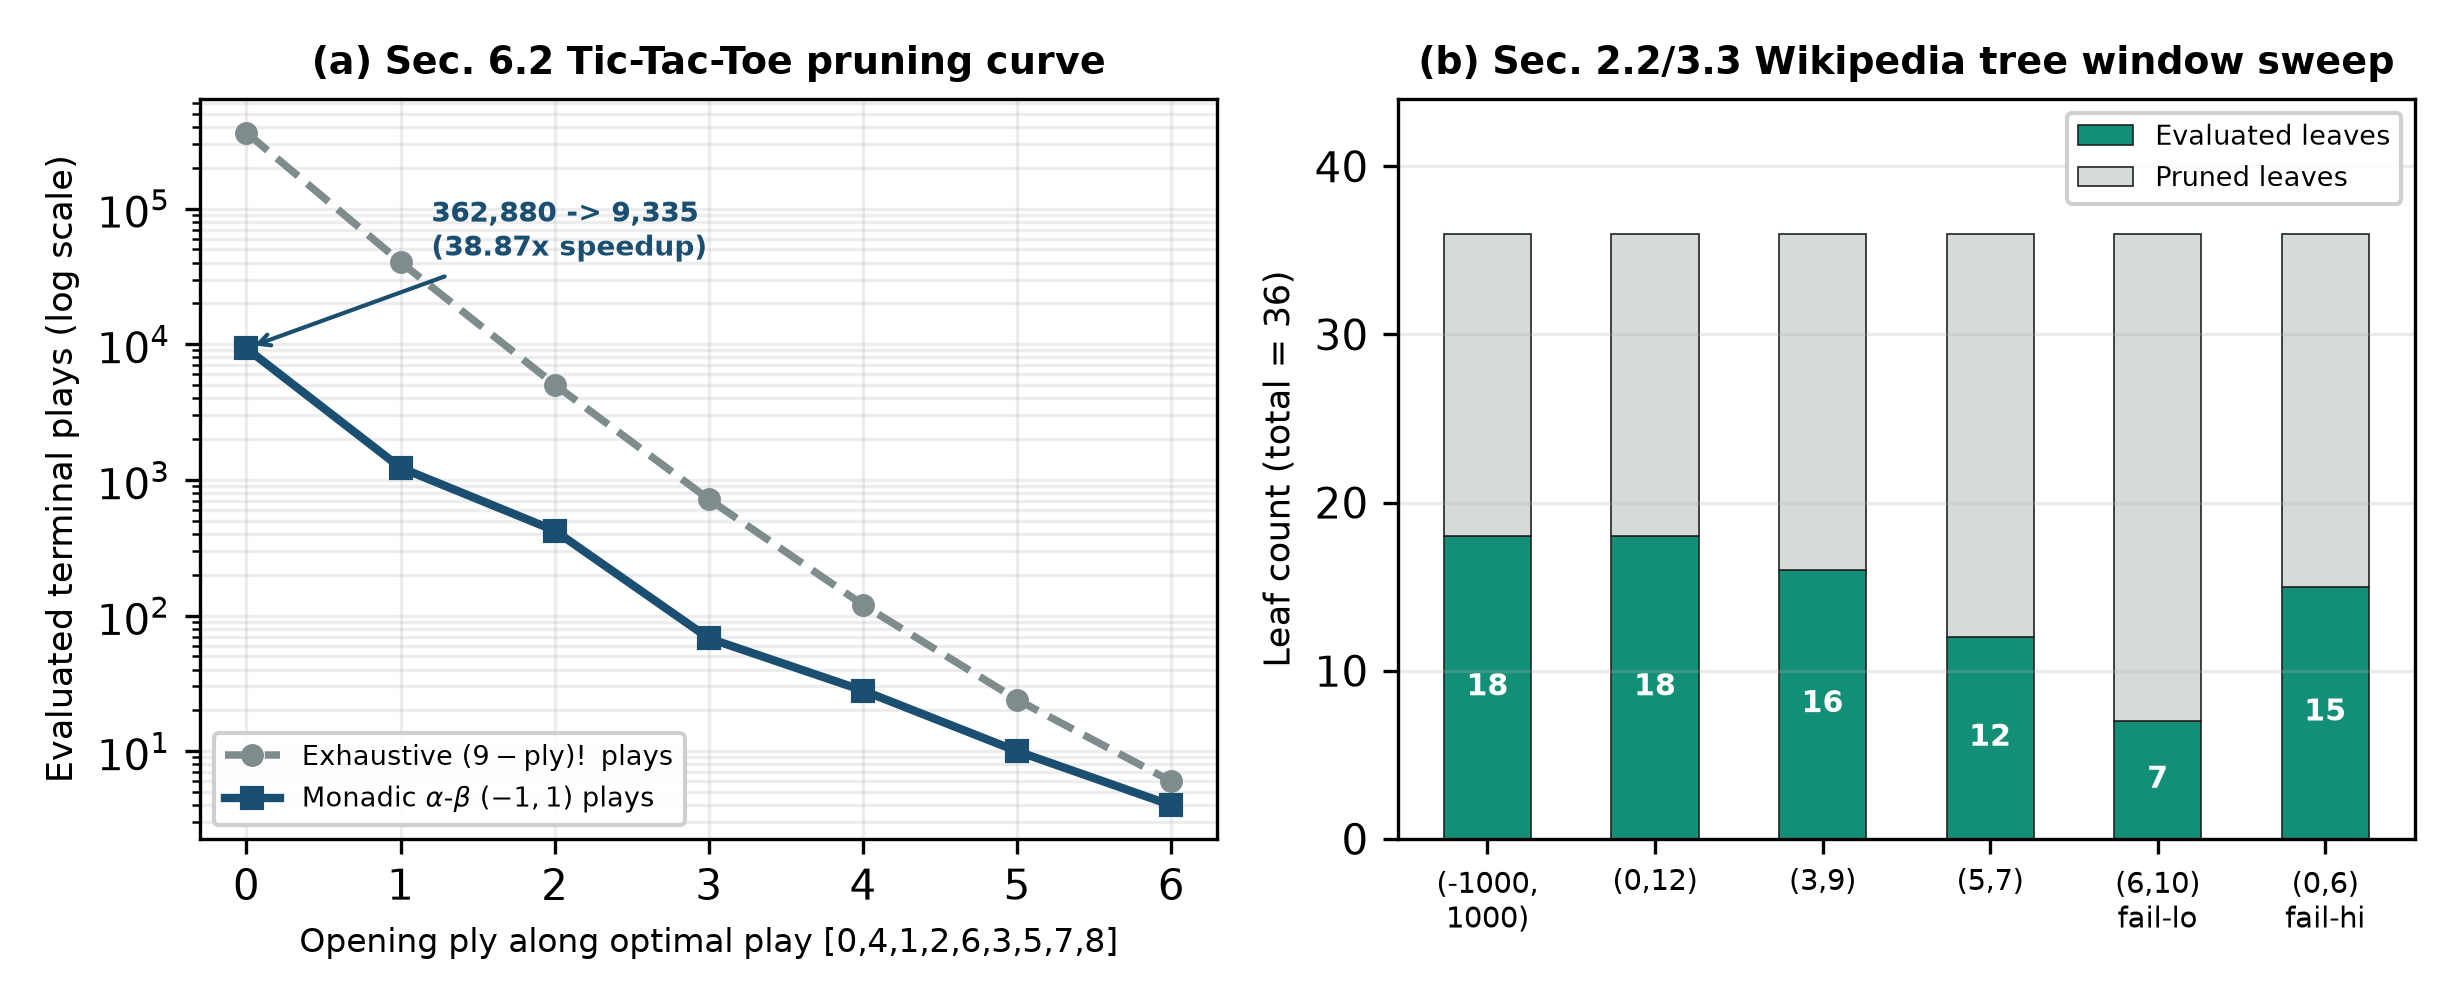
\includegraphics[width=\columnwidth]{../figures/fig1_ttt_and_wiki_pruning.png}
  \caption{(a) Exact Tic-Tac-Toe evaluated plays along Escard{\'o} and Oliva's optimal draw line $[0,4,1,2,6,3,5,7,8]$ from ply~0 ($362{,}880 \to 9{,}335$, $38.873\times$) through ply~6 ($6 \to 4$). (b) Exact Wikipedia 36-leaf tree pruning across six windows centered on optimal value $6$.}
  \label{fig:ttt}
\end{figure}

\paragraph{Tic-Tac-Toe \& Window Sensitivity (Fig.~\ref{fig:ttt}).}
Mode~4 ($1.892$--$103.002\,\mathrm{ms}$) reproduces Escard{\'o} and Oliva's exact Section~6.2 full-root Tic-Tac-Toe benchmark under $(-1,1)$: $9! = 362{,}880$ full plays collapse to $9{,}335$ evaluated plays ($38.873\times$ speedup), returning exact draw value $0$ and optimal play $[0,4,1,2,6,3,5,7,8]$. Along its prefixes, pruning achieves $32.780\times$ at ply~1 ($40{,}320 \to 1{,}230$), $11.915\times$ at ply~2 ($5{,}040 \to 423$), $10.588\times$ at ply~3 ($720 \to 68$), $4.286\times$ at ply~4 ($120 \to 28$), and certifies an X-win subgame $[0,1,4]$ ($720 \to 137$, value $+1$ under $(-2,2)$). On the Wikipedia 36-leaf tree, tightening the window from $(-1000,1000)$ to $(3,9)$ and $(5,7)$ reduces evaluated leaves from $18$ to $16$ and $12$, while fail-low $(6,10)$ and fail-high $(0,6)$ prune to $7$ and $15$ leaves.

\begin{figure}[t]
  \centering
  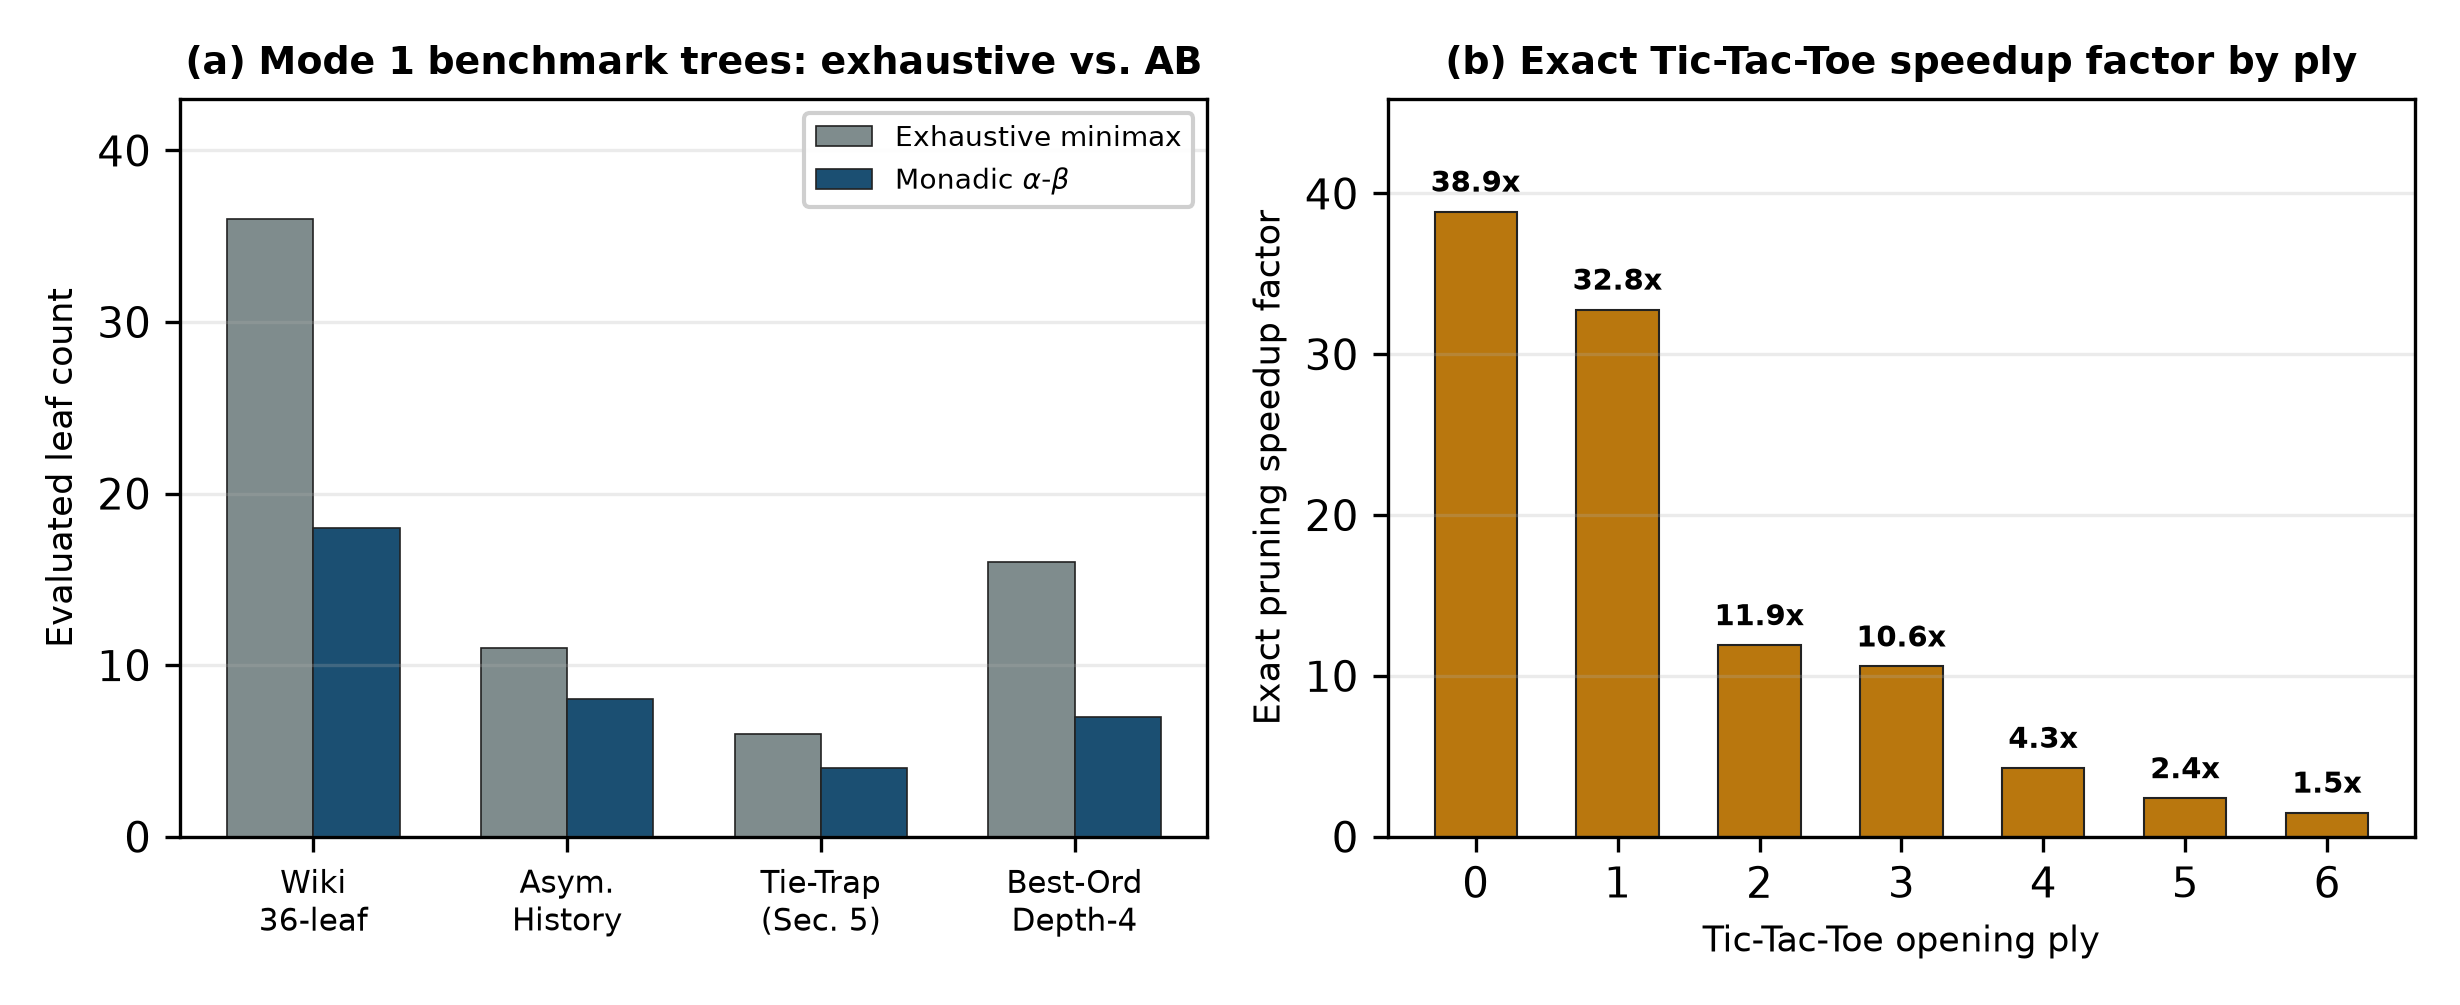
\includegraphics[width=\columnwidth]{../figures/fig2_benchmarks_and_speedup.png}
  \caption{(a) Exhaustive versus monadic alpha-beta evaluated leaves across all four Mode~1 benchmark trees. (b) Exact speedup ratio $(9-\mathrm{ply})! / \mathrm{ab\_leaves}$ across Tic-Tac-Toe plies $0$--$6$.}
  \label{fig:bench}
\end{figure}

\paragraph{Fixed-Tree Benchmarks \& Optimal Plays (Fig.~\ref{fig:bench}).}
Mode~1 ($0.093$--$0.344\,\mathrm{ms}$) certifies the exact Wikipedia tree ($36 \to 18$ leaves, value $6$, play $[1,0,0,0]$), an asymmetric history-dependent tree ($11 \to 8$, value $6$), the Section~5 tie-breaking trap ($6 \to 4$, value $5$, where first-element \texttt{pickMax} keeps $[0,1]$ over a pruned tied bound), and a best-ordered depth-4 binary tree ($16 \to 7$, value $6$). Mode~2 ($0.118$--$0.398\,\mathrm{ms}$) checks 17 windows covering all three Theorem~1 regimes across the four trees, and Mode~3 ($0.092$--$0.305\,\mathrm{ms}$) certifies ply-by-ply Definition~2 optimality for every extracted play.

\begin{figure}[t]
  \centering
  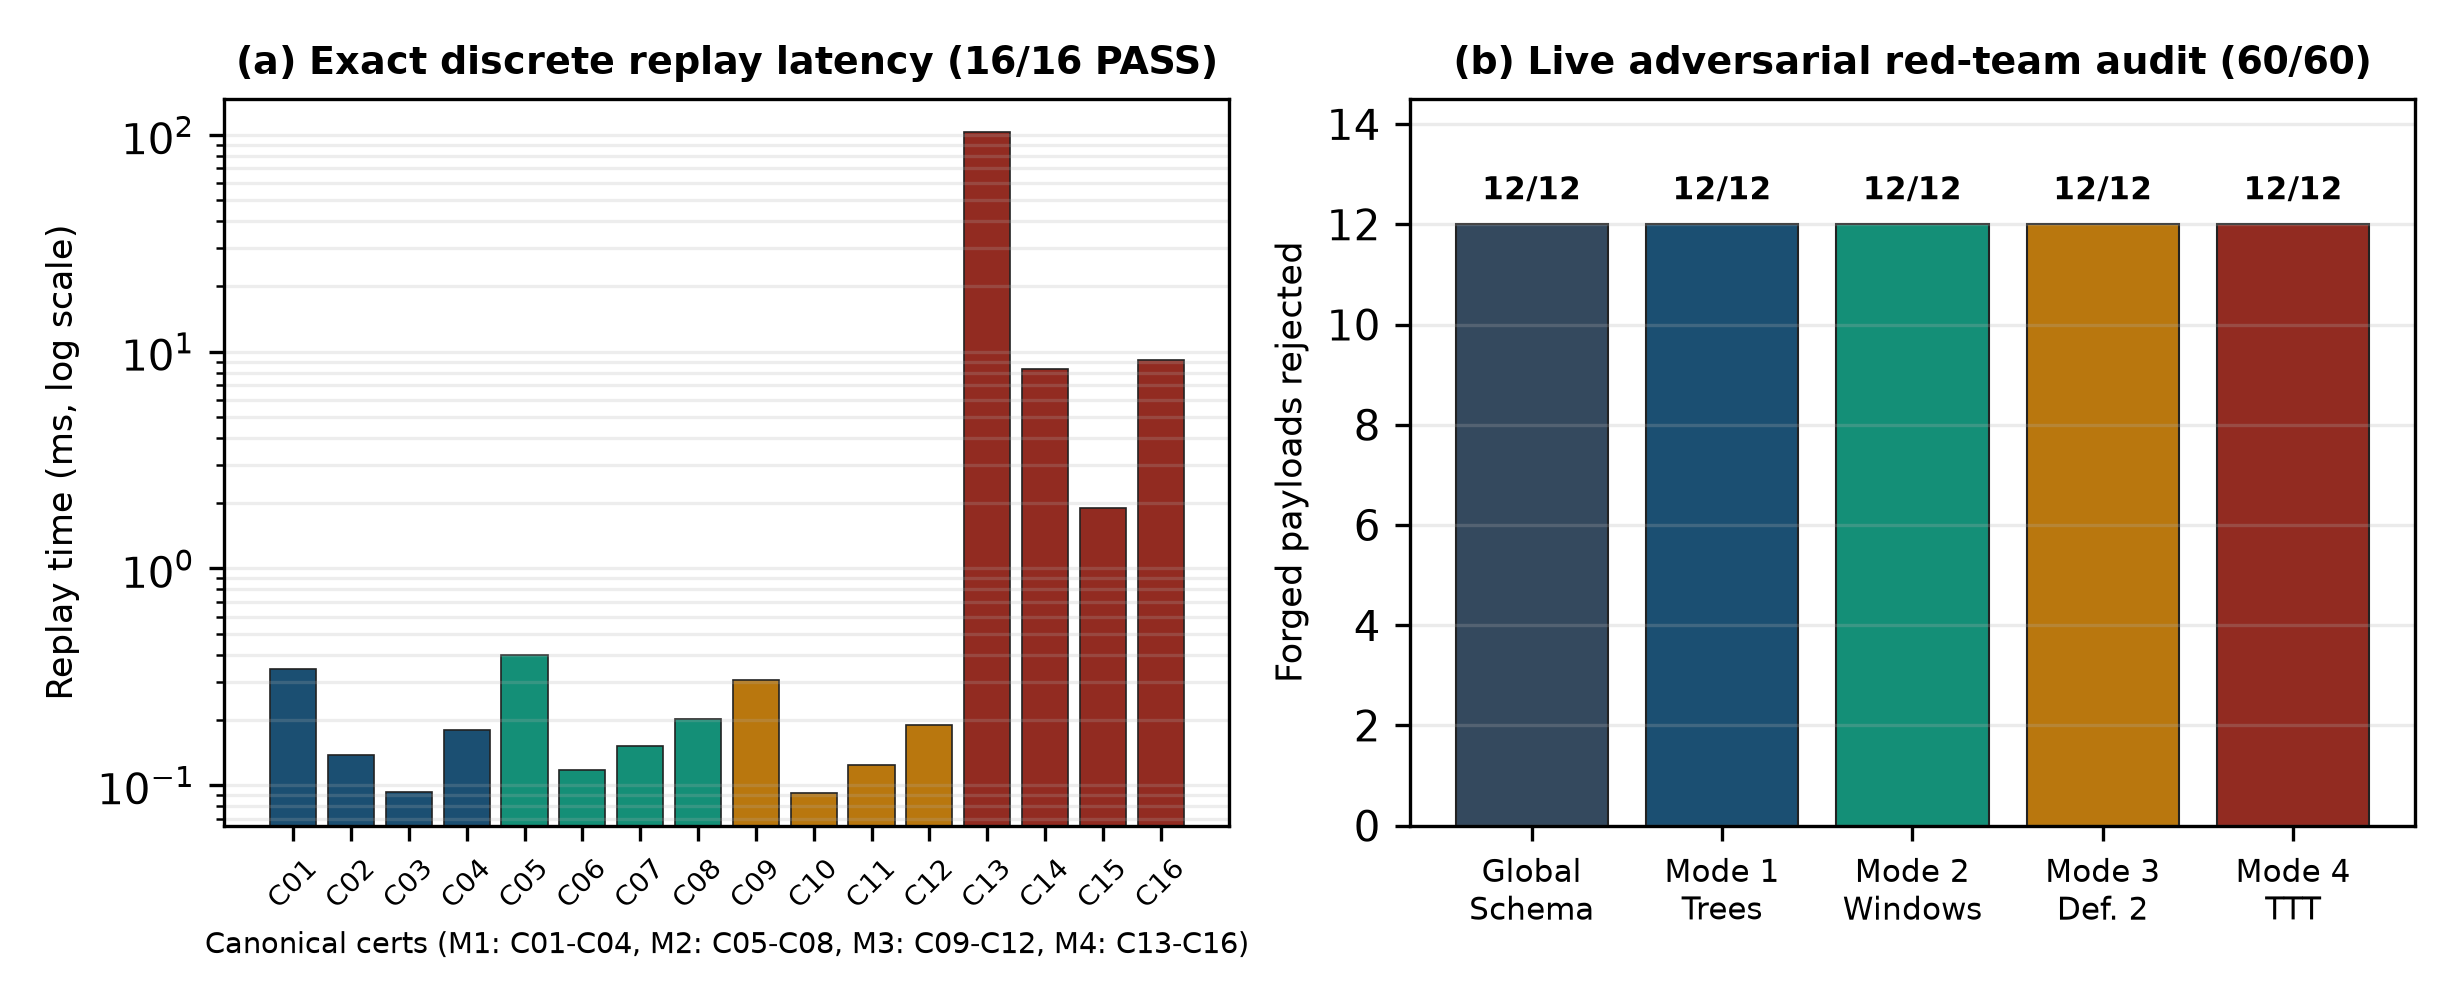
\includegraphics[width=\columnwidth]{../figures/fig3_certificate_replay_atlas.png}
  \caption{(a) Exact discrete replay latency ($0.092$--$103.002\,\mathrm{ms}$) across all 16 canonical \texttt{ALPHABETA-MONAD-CERT-1.0} certificates. (b) Live adversarial red-team audit rejecting 60/60 forged payloads across all five categories.}
  \label{fig:atlas}
\end{figure}

\paragraph{Replay Latency and 60/60 Red-Team Audit (Fig.~\ref{fig:atlas}).}
All 16 canonical certificates replay deterministically in $0.092$--$103.002\,\mathrm{ms}$ (total $124.66\,\mathrm{ms}$; $0.092$--$0.398\,\mathrm{ms}$ for Modes~1--3 and $1.892$--$103.002\,\mathrm{ms}$ for Mode~4). The live adversarial suite (\texttt{tests/test\_suite.py}) executes 60 targeted forgeries---12 global schema/typing/depth/control-char attacks plus 12 domain attacks per mode (invalid tree nodes, duplicate moves, $\alpha \ge \beta$, tampered leaf traces, misclassified Theorem~1 regimes, tie-breaking trap swaps, non-optimal plays, illegal/duplicate Tic-Tac-Toe moves, and corrupted $9{,}335$ leaf counts)---achieving \textbf{60/60 (100\%)} rejection.

\section{Conclusion}\label{sec:conc}
We delivered a standalone, zero-floating-point verification framework for Escard{\'o} and Oliva's monadic continuation alpha-beta theory~\cite{escardo2026alphabeta}, combining 18 zero-\texttt{sorry}, zero-\texttt{Classical.choice} Lean~4.35.0 theorems with the exact discrete verifier \texttt{ALPHABETA-MONAD-CERT-1.0}, 16 canonical certificates (including exact $362{,}880 \to 9{,}335$ Tic-Tac-Toe), and 60/60 live adversarial forgery rejections.

\bibliographystyle{plain}
\bibliography{references}
\end{document}
